\section{Google Cloud Function}

O Google Cloud Functions se qualifica como uma forma simples de executar código
em nuvem, fazendo escalonamento automático com alta tolerância a falhas que
dispensa provisionamento e configurações de servidor e oferece cobrança somente
quando o o código esta em execução.

\subsection{Propósito}

De acordo com a documentação da Google, os principais propósitos do Cloud
Functions são, entregar ao desenvolvedor uma plataforma leve para criar funções
independentes que respondam a eventos da nuvem sem necessidade de gerenciar
servidores e ambientes de execução.

Os principais tipos de aplicação pensados para funcionar com essa estrutura
são, \textit{back-end} de aplicações sem servidor como sites e aplicativos,
processamento de dados, arquivos, \textit{streams} e processos de ETL, além de
aplicativos inteligentes, como assistentes virtuais, \textit{chatbots}, analise
de video, imagens e analise de sentimento.

\subsection{Implantação}
Para a implantação de um novo código para automação, processamento ou outro
proposito, deve-se pensar não a nível de sistema, mas de funções isoladas com
comportamentos finalidade única e bem estabelecida.

\bigskip
Cada uma dessas funções ou comportamentos deve ser escrita na linguagem
escolhida dentre uma curta lista de opções.

\bigskip
De acordo com o passo-a-passo da Google, para implantar uma função no Cloud
Functions deve-se seguir 5 passos:
\begin{alineas}
	\item Preparação
	\item Criar uma Cloud Function
	\item Escrever o código da função
	\item Testar a função
	\item Escrever o código da função
	\item Observar registros
\end{alineas}

A etapa de preparação que consiste na habilitação de cobrança e permissões no
Google não é relevante do ponto de vista de comparação com o nosso projeto,
entretanto a partir do segundo item, a relevância passa a existir.
Criar uma Cloud Function é uma etapa de configuração e ao mesmo tempo de
implantação da função que será escrita para o ambiente. Essas configurações
abrangem um nome para a função, a quantidade máxima de memória que será
alocada, um gatilho para a função que pode vir de múltiplos serviços oferecidos
pela nuvem do Google, requisições HTTP e HTTPS. Após a execução desses passos a
função está no ar e pronta para responder ao gatilho definido.

\bigskip
A proposta principal desse serviço não é ter uma flexibilidade incrível de
configurações e nem garantir uma quantidade enorme de recursos para uma função,
mas oferecer um meio simples e rápido de implementar uma função e
disponibiliza-la para uso sem a necessidade de gerenciar servidores e ambientes
de execução.

\subsubsection{Entrada e saída}

O Google Cloud Functions é bastante limitado em relação a interfaces de entrada
e saída. Os possíveis meios entradas são pre-estabelecidos e normalmente são
serviços da própria nuvem do Google. No contexto do Cloud Functions as entradas
são tradas como \textit{triggers} (gatilhos) e elas estão listadas na Fig.
\ref{fig:google-cloud-functions-triggers}. Além disso, no caso das saídas, elas
estão restritas somente a execuções de procedimentos sem respostas por parte da
função ou como única forma de saída através de respostas a requisições HTTP, ou
seja, somente funcionam para gatilhos HTTP.

\bigskip
Além das restrições em relação a interface de entrada e de saída, existem ainda
restrições em relação as definições de segurança. Se um desenvolvedor escolhe
HTTP como gatilho de entrada por exemplo, ele só pode funcionar através de
HTTPS com TLS configurado pela Google, ou seja inviabiliza uso de autenticação
\textit{Client Certificate} (certificados do cliente) por exemplo.

\begin{figure}[ht]
	\centering
	\caption{Gatilhos permitidos}

	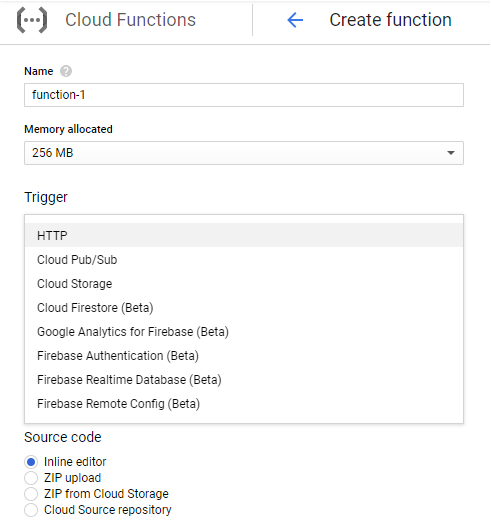
\includegraphics[width=12.5cm]{figuras/google-cloud-functions/triggers.png}
	\legend{Fonte: cloud.google.com/functions/}
	\label{fig:google-cloud-functions-triggers}
\end{figure}

\bigskip
Ou seja, apesar da versatilidade e facilidade de usar Google Cloud Functions,
ela vem associada a muitas restrições de entrada e saída e também customizações
de segurança.

\subsubsection{Linguagens}

Para os procedimentos e funções rodando no Cloud functions existe uma lista de
possíveis linguagens de programação disponíveis, dentre essas linguagens temos
Node.js, Python e Go.
Para o Node.js estão disponiveis as versões \textbf{Node.js 6} (deprecada),
\textbf{Node.js 8}, \textbf{Node.js 10}, Para Python somente a versão
\textbf{Python 3.7.1} e para Go somente \textbf{Go 1.11.65}.

\subsubsection{Escalabilidade}

O Cloud functions possui mecanismos de auto escalabilidade onde mais instâncias
são recrutadas para tratar um fluxo maior de requisições, isso possibilita que
a função implantada tenha bastante espaço para escalabilidade. Entretanto, a
Google desenhou o sistema de forma que cada instancia trata somente uma
requisição por vez, sem espaço para requisições assincronas, ou concorrentes em
um mesmo nó. De acordo com a Google, isso garante que a instância tenha todo o
CPU e memória reservados para sua execução, sem a necessidade de
compartilhamento. Entretanto, esse mecanismo pode gerar desperdicio de CPU e
memória ociosos. O Google garante que conforme mais requisições chegarem ao
sistema, mais instâncias serão recrutadas para atenderem a demanda. Entretanto,
para cada instancia iniciada, existe um processo de \textit{could start} que
pode fazer com que requisições que atingiram instâncias em periodo de start
possam demorar significativamente mais que requisições que atingiram instâncias
já rodando dependendo do tempo de inicialização da função em questão.

\bigskip
A escalabilidade do Cloud functions também possui algumas configurações
disponíveis para o desenvolvedor, como por exemplo, o numero máximo de
instâncias permitido. De acordo com o Google, essa funcionalidade serve para
limitar por exemplo numero de instâncias acessando um banco de dados, ou algum
outro recurso limitado, evitando assim acessos acessivos,

\bigskip
Outro aspecto relevante para a escalabilidade são as circunstancias nas quais
uma nova instância é recrutada, e existem essencialmente dois casos:
\begin{alineas}
	\item Quando uma nova função é implantada no Cloud functions:
	\item Quando o numero de requisições em andamento simultaneamente é
	maior que o número de instâncias e menor que o número máximo de
	instâncias
	pré-configurado.
\end{alineas}

\bigskip
De acordo com a documentação, uma mesma instância pode ser usada muitas outras
vezes após sua inicialização e quando possível a função deve fazer
\textit{cache} para economizar tempo de execução. Além disso, deve se tomar
cuidado quanto a erros ocorrendo nas funções, uma vez que as duas razões para
uma instância ser desativada são, erros irrecuperáveis e trafego baixo.

\subsubsection{Flexibilidade}

Apesar do Cloud functions oferecer algumas configurações e facilidades, o
sistema também cria algumas limitações. Nesse sentido, alguns aspectos como
tempo de execução, sistema de arquivos, rede, entrada e saída de dados, devem
ser observados com cautela. O tempo máximo de execução de uma função é
configurável, entretanto, o limite máximo permitido são 9 minutos. Quanto ao
sistema de arquivos, ele será composto pelo arquivo da função em questão e suas
dependências, entretanto, todo o sistema de arquivos dará a função somente
permissão de leitura, exceto no diretório /tmp. Entretanto o diretório /tmp
deve ser usado com cautela, uma vez que o espaço consumido nesse diretório na
realidade é alocado na memória principal, e pode consumir recursos necessários
para a execução da função. Quanto a rede, a função não pode fazer acessos de
rede local, mas possui acesso a internet. No contexto de internet e
requisições, deve-se ficar atento, uma vez que qualquer conexão que dure mais
que 2 minutos é automaticamente desfeita pela Google gerando \textit{socket
	hangup} para a outra parte envolvida. Quanto a entrada de dados, a
lista da
Fig. \ref{fig:google-cloud-functions-triggers} mostra as poucas alternativas
fornecidas. Já com relação a saída, no caso de eventos, a saída pode acontecer
de qualquer maneira permitida que necessite acesso a internet, entretanto para
gatilhos em HTTP, somente uma resposta HTTP pode ser dada.

\subsection{Arquitetura}

https://cloud.google.com/functions/quotas

TODO
\begin{figure}[ht]
	\centering
	\caption{Diagrama de funcionamento}

	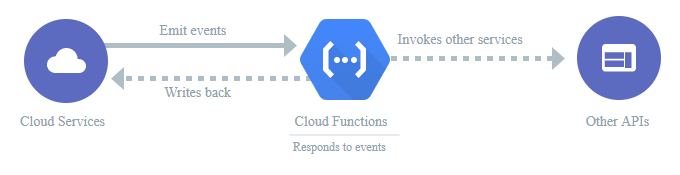
\includegraphics[width=12.5cm]{figuras/google-cloud-functions/workflow.png}
	\legend{Fonte: console.cloud.google.com}
	\label{fig:google-cloud-functions-workflow}
\end{figure}

\subsubsection{Protocolos de rede}

TODO

\subsubsection{Tolerância à falhas}

TODO

\subsection{Licença}

TODO

\subsection{Preço}

TODO

\subsection{Comparação}

TODO
